\documentclass[11pt,a4paper]{report}

\usepackage{polski}
\usepackage[utf8]{inputenc} 
\usepackage{a4wide}
\usepackage{tabularx}
\usepackage{lastpage}
\usepackage{fancyhdr}
\usepackage{graphicx}
\usepackage{caption}

% strona tytułowa
\begin{titlepage}
\title{\Huge Sprawozdanie z Projektu\\\textsl{The Game of Life}}
\author{Daniel Ślusarczyk i Jakub Łaba}
\date{07.04.2021}
\end {titlepage}

\renewcommand{\footrulewidth}{0pt}
\begin{document}
\maketitle

% zmiana numeracji sekcji 0.X -> X
\renewcommand*\thesection{\arabic{section}} 
\begin{abstract}
Dokument stanowi sprawozdanie z projektu \textsl{"The Game of Life"}, z wyszczególnionym opisem aktualnego stanu projektu, zmian względem specyfikacji oraz wnioskami.
\end{abstract}

% numeracja stron
\pagestyle{fancy}
\fancyhf{}
\rhead{\textsl{Sprawozdanie z projektu "The Game of Life" | D. Ślusarczyk, J. Łaba}}
\rfoot{Strona \thepage \hspace{1pt} z \pageref{LastPage}}
\setcounter{page}{0}

% spis treści bez numeracji stron
\fancypagestyle{plain}
{
\fancyhead{} 
\fancyfoot{} 
}
\thispagestyle{empty} 
\tableofcontents 
\thispagestyle{empty}
\newpage

\fancypagestyle{plain} 
{
\fancyhead{} 
\fancyfoot[C]{\thepage}
}


% pierwsza sekcja
\section{Zarys Projektu}\label{sec:tekst}
Projekt \textsl {„The Game of Live”} zakłada stworzenie programu emulującego działanie automatu komórkowego Johna Conwaya -- Grę w Życie (ang. The Game of Life), oraz napisanie dokumentacji opisującej stronę funkcjonalną i implementacyjną programu. Działanie gry jest następujące: na prostokątnej planszy znajdują się komórki żywe oraz martwe. Program przeprowadza określoną liczbę generacji, w których komórki ożywają/obumierają na następujących zasadach:
\begin {itemize}
\item\textbf {Komórki żywe} -- pozostają żywe w kolejnej generacji, jeżeli posiadają dokładnie 2 lub 3 żywych sąsiadów, w każdym innym przypadku umierają.
\item\textbf {Komórki martwe} -- ożywają w kolejnej generacji, jeżeli posiadają dokładnie trzech żywych sąsiadów, w przeciwnym przypadku pozostają martwe.
\end {itemize}
Komórki znadujące się poza planszą są uznawane za permanentnie martwe.


% druga sekcja
\section{Struktura programu}\label{sec:tekst}
\subsection {Struktura katalogów}
Projekt został podzielony na 3 katalogi dla zachowania porządku w jego plikach. Katalog \textsl{kod} zawiera cały kod źródłowy projektu oraz skrypt makefile. Katalog \textsl{dokumenty} -- całą dokumentację projektu, natomiast \textsl{input} przykładowe pliki wejściowe do uruchomienia programu.
\subsection {Struktura modułów}
Program składa się z trzech modułów: \textsl{tgol\_file}, \textsl{tgol\_evo}, \textsl{tgol\_png} oraz pliku \textsl{tgol\_main.c}, zawierającego funkcję main całego programu oraz kluczowe makra.
Każdy z modułów składa się z dwóch plików: .h oraz .c, o odpowiedniej nazwie. W każdym z modułów plik .h zawiera prototypy funkcji oraz ewentualne definicje struktur, stałe oraz makra.
Większość obsługi błędów znajduje się bezpośrednio w funkcji main, z tego względu, że gdyby zostały przeniesione do zewnętrznych funkcji, niezbędne byłoby przekazywanie dużej ilości parametrów -- byłoby to niezbyt czytelne. Drugą możliwością byłoby zadeklarowanie owych zmiennych jako globalne, jednak duża ilość zmiennych globalnych nie jest dobrą praktyką.
Moduł tgol\_file zawiera funkcje odpowiadającą za wczytanie zawartości plików tekstowych do macierzy w formacie CRS oraz za zapis końcowego stanu planszy do plików tekstowych. Zawiera również definicje kodów błędów oraz pomocnicze struktury, pozwalające na wyświetlanie komunikatów o błędach oraz sprawdzanie flag.
Moduł tgol\_evo zawiera funkcje związane z przeprowadzaniem ewolucji -- tj. wyświetlanie macierzy na podstawie CRS na ekran oraz przekształcanie CRS zgodnie z jednym z dwóch sąsiedztw, oraz zasadami \textsl{"The Game of Life"}. Ponadto w module znajdują się funkcje pomocnicze, dla tych dwóch głównych funkcjonalności.
Moduł tgol\_png zawiera funkcje związane z generowaniem plików graficznych w formacie .png na podstawie macierzy w formacie CRS.
\begin{figure}[!ht]
\centerline{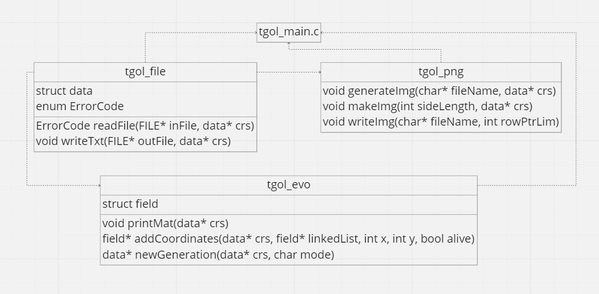
\includegraphics{img/diagram.png}}
\caption{Diagram modułów}
\end{figure}
\newpage



% trzecia sekcja
\section{Kompilacja programu}
Skrypt makefile został wyposażony w 4 opcje:
\begin{itemize}
\item\subsubsection{Domyślna kompilacja -- make} Kompiluje program w wersji dla użytkownika z zastosowaniem sąsiedztwa Moore'a.
\item\subsubsection{Kompilacja z sąsiedztwem von Neumanna -- make neumann} Kompiluje plik w wersji dla użytkownika z zastosowaniem sąsiedztwa von Neumanna.
\item\subsubsection{Kompilacja w trybie debug -- make debug} Kompiluje program z dodatkowymi informacjami, przydatnymi do debugowania oraz flagą -g, aby umożliwić analizę za pomocą programów \textsl{gdb} oraz \textsl{valgrind}.
\item\subsubsection{Skasowanie plików -- make clean} Kasuje plik wykonywalny oraz wszystkie pliki obiektowe.
\end{itemize}
\newpage

% czwarta sekcja
\section{Przykładowe wyniki działania programu}\label{sec:teskt}
Przedstawione poniżej wyniki programu prezentują różne kombinacje flag z różnymi plikami w celu zarysowania możliwości działania programu.
\begin {itemize}
\item \subsubsection {Podstawowe uruchomienie}
\subsubsection {Plik wejściowy}
\textsl{Rysunek 2} przedstawia plik wejściowy zawierający 5 punktów rozmieszczonych na planszy 10 na 10 tzw. \textsl{szybowiec}.
\begin{figure}[!ht]
\centerline{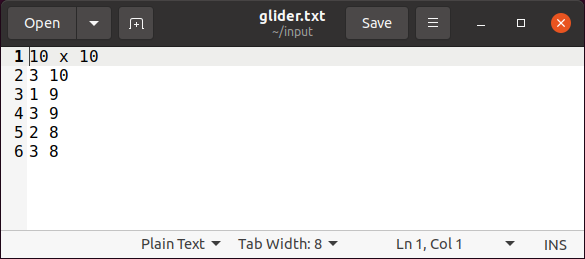
\includegraphics{img/input_glider.png}}
\caption{Plik wejściowy glider.txt}
\end{figure}
\subsubsection {Wywołanie:}
\texttt{./TGOL ../input/glider.txt 3}
\subsubsection {Wynik działania}
\textsl{Rysunek 3} przedstawia wynik działania programu zawierającego zadaną liczbę generacji wypisanych jedną pod drugim.
\begin{figure}[!ht]
\centerline{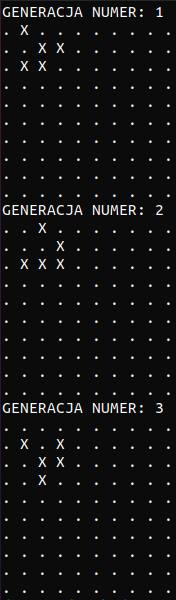
\includegraphics{img/output_glider.png}}
\caption{Wynik działa programu}
\end{figure}
\newpage

\item \subsubsection {Uruchomienie z flagą  \textsl{\textbf{-refresh}} bez parametru}
\subsubsection {Plik wejściowy}
\textsl{Rysunek 4} przedstawia plik wejściowy zawierający 6 punktów rozmieszczonych na planszy 6 na 6 tworzący układ, który powtarza się co dwie generacje.
\begin{figure}[!ht]
\centerline{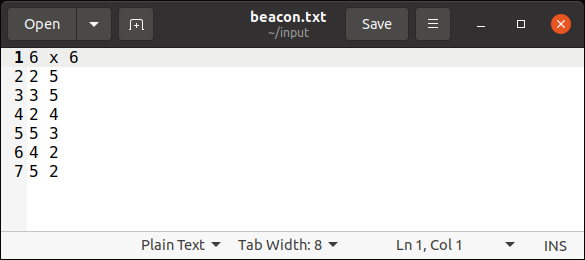
\includegraphics{img/input_beacon.png}}
\caption{Plik wejściowy beacon.txt}
\end{figure}
\newpage
\subsubsection {Wywołanie:}
\texttt{./TGOL ../input/beacon.txt 10 -refresh}
\subsubsection {Wynik działania}
\textsl{Rysunki 5 i 6} przedstawiają wynik działania programu, który w pierwszym etapie informuje o wybraniu podstawowej częstotliwości odświeżania, a następnie wyświetla kolejne generacje w podanym odstępie, kończąc działania na ostatniej generacji w etapie drugim.
\begin{figure}[!ht]
\centerline{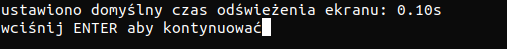
\includegraphics{img/output_beacon1.png}}
\caption{Wynik działa programu w etapie pierwszym}
\end{figure}
\begin{figure}[!ht]
\centerline{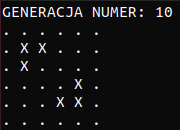
\includegraphics{img/output_beacon2.png}}
\caption{Wynik działa programu w etapie drugim}
\end{figure}

\item \subsubsection {Uruchomienie z flagą  \textsl{\textbf{-refresh}} z parametrem oraz flagą  \textsl{\textbf{-sbs}}}
\subsubsection {Plik wejściowy}
\textsl{Rysunek 7} przedstawia plik wejściowy zawierający 18 punktów rozmieszczonych na planszy 10 na 20.
\begin{figure}[!ht]
\centerline{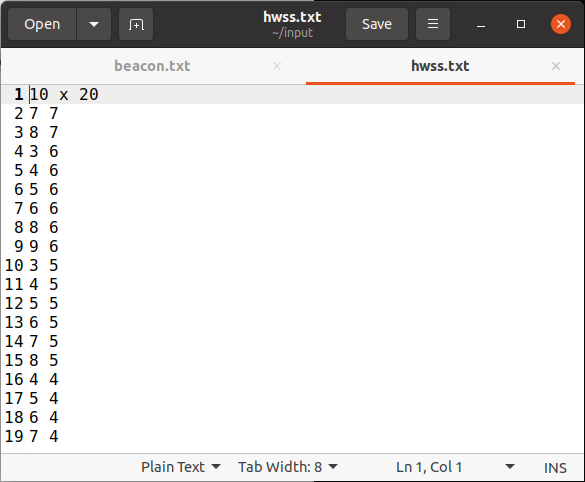
\includegraphics{img/input_hwss.png}}
\caption{Plik wejściowy hwss.txt}
\end{figure}
\subsubsection {Wywołanie:}
\texttt{./TGOL ../input/hwss.txt 10 -refresh 0.5 -sbs}
\subsubsection {Wynik działania}
\textsl{Rysunki 7, 8 i 9} przedstawiają wynik działania programu, który w pierwszym etapie informuje o częstotliwości odświeżania, a następnie w każdym kolejnym etapie wyświetla kolejne generacje, czekając na przycisk.
\begin{figure}[!ht]
\centerline{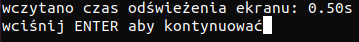
\includegraphics{img/output_hwss1.png}}
\caption{Wynik działa programu w etapie pierwszym}
\end{figure}
\begin{figure}[!ht]
\centerline{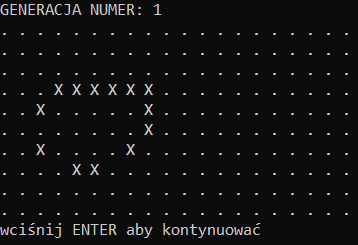
\includegraphics{img/output_hwss2.png}}
\caption{Wynik działa programu w etapie drugim}
\end{figure}
\begin{figure}[!ht]
\centerline{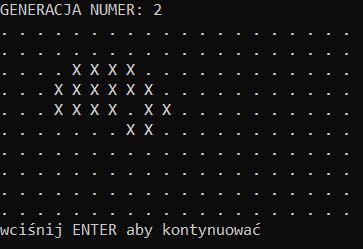
\includegraphics{img/output_hwss3.png}}
\caption{Wynik działa programu w etapie trzecim}
\end{figure}

\item \subsubsection {Uruchomienie z flagą  \textsl{\textbf{-refresh}} z parametrem oraz flagą  \textsl{\textbf{-save}}}
\subsubsection {Plik wejściowy}
\textsl{Rysunek 11} przedstawia plik wejściowy zawierający 36 punktów rozmieszczonych na planszy 40 na 40.
\begin{figure}[!ht]
\centerline{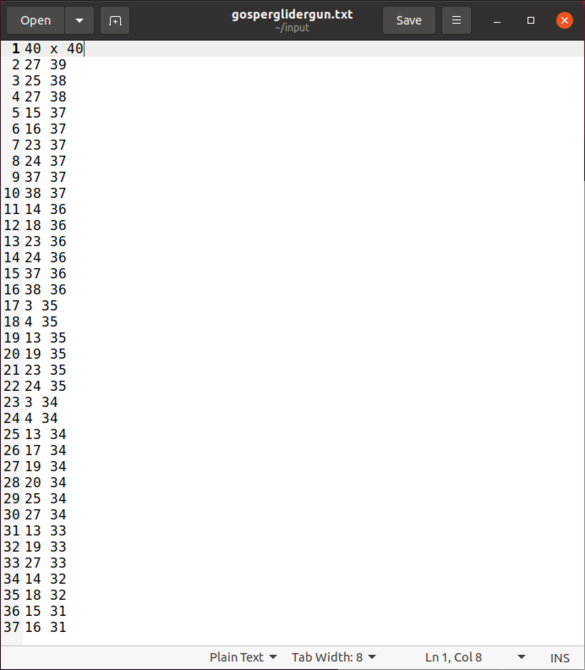
\includegraphics{img/input_gosperglidergun.png}}
\caption{Plik wejściowy gosperglidergun.txt}
\end{figure}
\subsubsection {Wywołanie:}
\texttt{./TGOL ../input/gosperglidergun.txt 100 -refresh 0.05 -save out}
\subsubsection {Wynik działania}
\textsl{Rysunki 12 i 13} przedstawiają wynik działania programu, który w pierwszym etapie informuje o wybraniu podanej częstotliwości odświeżania, a następnie wyświetla kolejne generacje w podanym odstępie, kończąc wyświetlanie generacji w drugim etapie. W ostatnim kroku program generuje plik tekstowy z rozszerzeniem \textsl{.txt} (\textsl{Rysunek 14}) i plik graficzny z rozszerzeniem \textsl{.png} (\textsl{Rysunek 15}) na podstawie ostatniej generacji.
\begin{figure}[!ht]
\centerline{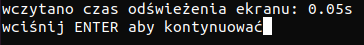
\includegraphics{img/output_gosperglidergun1.png}}
\caption{Wynik działa programu w etapie pierwszym}
\end{figure}
\begin{figure}[!ht]
\centerline{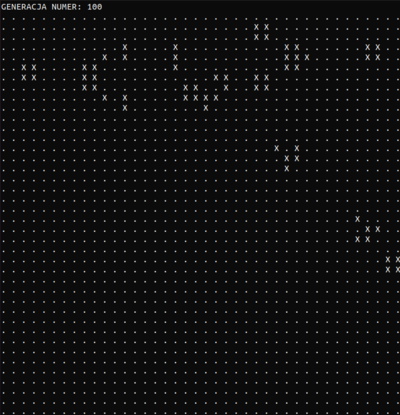
\includegraphics{img/output_gosperglidergun2.png}}
\caption{Wynik działa programu w etapie drugim}
\end{figure}
\begin{figure}[!hp]
\centerline{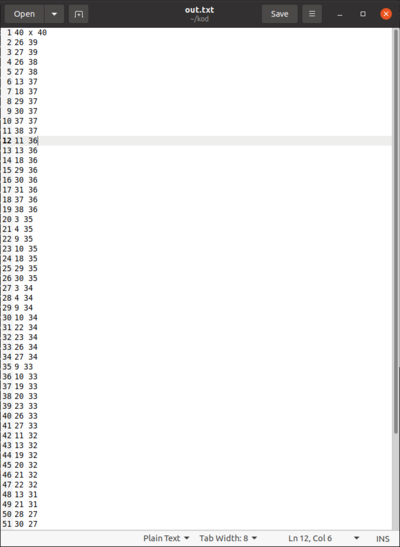
\includegraphics{img/output_gosperglidergun4.png}}
\caption{Wynik działa programu --plik tekstowy}
\end{figure}
\begin{figure}[!ht]
\centerline{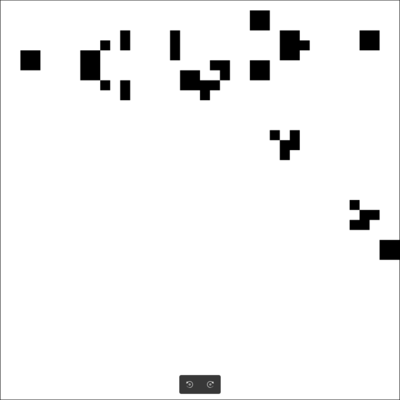
\includegraphics{img/output_gosperglidergun3.png}}
\caption{Wynik działa programu --plik graficzny}
\end{figure}
\end {itemize}
\newpage


% piąta sekcja
\section{Zmiany względem specyfikacji}\label{sec:teskt}
Założeniem projektu od samego początku powstawania było zachowanie ścisłości między pisanym programem, a specyfikacją funkcjonalna i implementacyjną. Proces powstawania elementów projektu zweryfikował dokładnie wszystkie założone idee i spowodował zmianę następujących punktów w poszczególnych dokumentach:

\subsubsection {Zmiana formatu danych wejściowych}
Program potrzebuje danych z informacjami o stanie wejściowej planszy (generacji 0), oraz o liczbie generacji, którą użytkownik chce wygenerować. Plik wejściowy powinien zawierać informacje sformatowane następująco:\\
\texttt {[row] x [col]}\\
\texttt {[x1] [y1]}\\
\texttt {[x2] [y2]}\\
\texttt {   ...  }\\
\texttt {[xn] [yn]}\\
Gdzie:
\begin {itemize}
\item \texttt {row} -- liczba rzędów planszy
\item \texttt {col} -- liczba kolumn planszy
\item \texttt{x1, x2, ..., xn} -- współrzędne x-owe kolejnych żywych komórek
\item \texttt{y1, y2, ..., yn} -- współrzędne y-owe kolejnych żywych komórek
\end {itemize}
\textbf{Uwaga:} kolejność podawania współrzędnych żywych komórek jest ustalona od lewej do prawej i od góry do dołu i tylko w takiej kolejności jest akceptowana. W przypadku niespełnienia tego warunku, lub innych błędów w formacie są zwracane odpowiednie kody błędów. Współrzędne określa się względem klasycznego 2--wymiarowego kartezjańskiego układu współrzędnych, a punkty nie mogą się powtarzać.
\subsubsection {\textsl{Przykład}}
Chcąc wczytać planszę 2x3 z jedną żywą komórką w lewym górnym rogu, oraz jedną w prawym dolnym rogu, plik powinien wyglądać w następujący sposób: \\
\texttt {2 x 3} \\
\texttt {1 2} \\
\texttt {3 1} 

\subsubsection {Zmiana działania flagi \textsl{\textbf{-save}}}
\textsl{\textbf{-save}} --program wywołany z tą flagą zapisze do pliku wynikowego ostatnią przeprowadzoną generację, sformatowaną identycznie jak plik wejściowy (dzięki temu można użyć pliku wynikowego jako wejścia do kolejnego uruchomienia programu) oraz zdjęcie w formacie \textsl{png} ostatniej generacji. Nazwę pliku wynikowego należy podać bezpośrednio po fladze \textsl{\textbf{-save}}, w przypadku chęci zapisania pliku w innym folderze, należy podać jego nazwę razem z pożądaną ścieżką\\

\subsubsection {Usunięcie błędów INPUT\_NOT\_INT, INPUT\_SHORT, INPUT\_XY}
Błędy INPUT\_NOT\_INT, INPUT\_SHORT, INPUT\_XY w wyniku nowego formatu pliku wejściowego straciły użyteczność.

\subsubsection {Dodanie błędów \textbf{INPUT\_INCORRECT}, \textbf{INPUT\_DIMS}, \textbf{INPUT\_XY\_LIMIT}, \textbf{INPUT\_INCORRECT\_ORDER}}
Wprowadzenie nowego formatu wymusiło wprowadzenie następujących  błędów, które są zwracana w przypadku nieprawidłowego pliku wejściowego zgodnie z tabelą:\\
\begin{tabularx}{\textwidth}{  X|Xl  }
 \hline
 Komunikat                                   					& Przyczyna\\
 \hline \hline
			INPUT\_INCORRECT			&W pliku wejściowym liczba współrzędnych x nie jest równa y, plik zawiera znaki niebędące liczbami naturalnymi, lub plik nie zawiera informacji o żadnych punktach\\
 \hline
			INPUT\_DIMS				&W pliku wejściowym znajduje się niewłaściwie wymiary planszy (niezgodny z formatem lub brak wymiaru)\\
 \hline
			INPUT\_XY\_LIMIT				&W pliku wejściowym podano zbyt wielkie wartości współrzędny względem deklarowanych wymiarów\\
\hline
			INPUT\_INCORRECT\_ORDER		&W pliku wejściowym zastosowano niepoprawną kolejność współrzędnych lub wystąpiło powtórzenie\\
 \hline
\end{tabularx}

\newpage

% szósta sekcja
\section{Podsumowanie współpracy}\label{sec:teskt}
Współpraca w obrębie projektu przebiegała sprawnie i bez większych problemów. Wartym odnotowania współczynnikiem, który wpływał korzystnie na efektywność współpracy, było korzystanie systemu kontroli wersji. Z pomocą tego narzędzia wymiana aktualnymi wersjami programu i zarządzanie całą strukturą programu odbywało się efektywnie. Pomocne były też częste rozmowy z wyjaśnieniami zastosowanych rozwiązań, wspólne uzgadnianie podziału pracy i podobieństwo tworzenia kodu na poziomie konceptualnym. Jedynym czynnikiem czasami negatywnie wpływającym na współpracę było modyfikowanie kodu, którego nie jest się autorem. Mogło to powodować nieścisłości w kodzie i utratę pewności do prawidłowego działania danego fragmentu kodu. Podsumowując, współpraca projektowa była na zadowalającym poziomie pomimo drobnych problemów i pozwalała na wspólne uczenie się nowych rozwiązań. 

% siódma sekcja
\section{Podsumowanie projektu}\label{sec:teskt}
Projekt  \textsl{"The Game of Life"} został w całości przygotowany od 24.02.2021 do 07.04.2021. W ramach niego powstał działający program  \textsl{TGOL}, makefile,  specyfikacja funkcjonalna, specyfikacja implementacyjna oraz sprawozdanie końcowe. Przygotowane rozwiązanie implementuję różne flagi pomocne podczas analizowania kolejnych generacji, posiada prostą i intuicyjną obsługę oraz pozwala na efektywne sprawdzanie kolejnych generacji za sprawą zastosowania metody przechowywania macierzy rzadkich CRS. Dodatkowo przy wywołaniu możliwe jest użycie flagi \textsl{\textbf{-save}}, która pozwala na zapis ostatniej generacji w postaci \textsl{png}. Program \textsl{TGOL} został przetestowany pod kątem różnych błędów i nietypowych plików wejściowych. W konsekwencji jego działanie powinno być w znaczącej liczbie przypadków zgodne z oczekiwaniami. 

% ósma sekcja
\section{Wnioski}\label{sec:teskt}
Projekt \textsl{"The Game of Life"} jest zadaniem, który pozwala na różnorodne podejście do problemu i zaimplementowanie rozwiązań, które znacząco wpłyną na działanie programu. W przypadku \textsl{TGOL}, czyli oprogramowania, które może analizować duże zbiory danych pomocne, jest zastosowanie narzędzia pozwalającego maksymalnie zmniejszyć używaną pamięć. Użyta w programie metoda \textsl{CRS} pozwoliła ograniczyć ten problem, ale jednocześnie negatywnie wpłynęła na czytelność i przejrzystość kodu. Ponadto przytoczony sposób reprezentacji macierzy rzadkiej utrudnia odwołanie się do elementów zerowych. Drugim istotnym aspektem jest ograniczenie do zera tzw.  \textsl{wycieków pamięci}, które w przypadku zastosowania języka C bywają ciężkie do wykrycia i naprawienia. Dla omawianego programu niezbędne okazało się użycia dodatkowych programów raportujących takie niezamierzone użycie pamięci. 


\end{document}